\documentclass{homework}
\usepackage{booktabs}
\usepackage{subfig}
\captionsetup[subfigure]{labelformat=empty}


\usepackage{tikz}
\usetikzlibrary{arrows}
\usetikzlibrary{matrix}

\usepackage{fancyvrb,newverbs,xcolor}

\definecolor{cverbbg}{gray}{0.93}

\newenvironment{cverbatim}
 {\SaveVerbatim{cverb}}
 {\endSaveVerbatim
  \flushleft\fboxrule=0pt\fboxsep=.5em
  \colorbox{cverbbg}{\BUseVerbatim{cverb}}
  \endflushleft
}
\newenvironment{lcverbatim}
 {\SaveVerbatim{cverb}}
 {\endSaveVerbatim
  \flushleft\fboxrule=0pt\fboxsep=.5em
  \colorbox{cverbbg}{%
    \makebox[\dimexpr\linewidth-2\fboxsep][l]{\BUseVerbatim{cverb}}
  }
  \endflushleft
}

\newcommand{\ctexttt}[1]{\colorbox{cverbbg}{\texttt{#1}}}
\newverbcommand{\cverb}
  {\setbox\verbbox\hbox\bgroup}
  {\egroup\colorbox{cverbbg}{\box\verbbox}}

\title{CIS 571 - Assignment 1}
\author{Ali Hassani}

\begin{document}

\maketitle

\renewcommand{\theenumi}{\alph{enumi}}
\renewcommand{\theenumii}{\roman{enumii}}

\exercise[1]
\subsection{Lonely bug}

\subsubsection{Environment}
The state could be represented by a $M \times N$ boolean matrix ($5 \times 5$ for this particular case), specifying whether each cell is accessible or not (walls, blocks, etc).
Therefore it could be represented either with an $M \times N$ boolean matrix.

\begin{figure}[h!]
    \centering
    \subfloat[\centering View]{{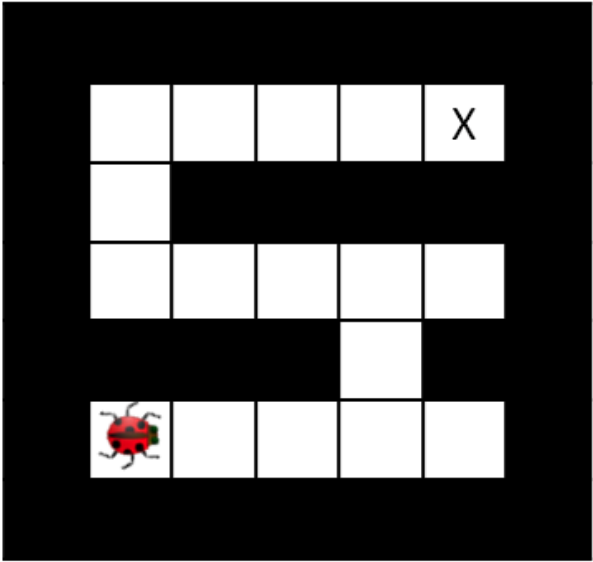
\includegraphics[width=0.25\textwidth]{figures/q11.png}}}
    \qquad
    \subfloat[\centering State grid]{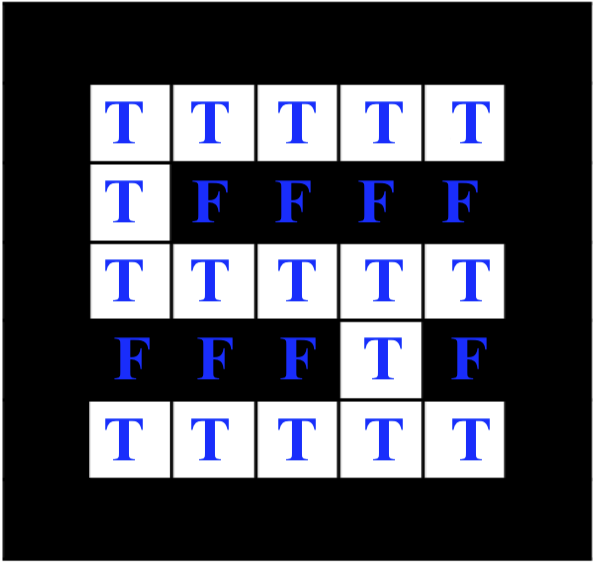
\includegraphics[width=0.25\textwidth]{figures/q11-sol.png}}
    \caption{Lonely bug map representation}
    \label{fig:lonelybug11}
\end{figure}

\subsubsection{States}
The insect's location and the target location could also be stored as two tuples separately (specifying the indices). They could be in any of the $MN$ cells in this particular game, which means there are $MN$ possible combinations for the bug state. Given that the number of walls within the map are exactly $P$, the number of bug states would come down to $MN - P$.

\subsubsection{Actions}
As for actions, the bug can take actions \textbf{stay}, \textbf{left}, \textbf{right}, \textbf{up} or \textbf{down}, only if they are legal (don't end up in a wall). It was not specified whether the bug can face a specific direction, therefore storing that in the state space can be excluded.

\subsubsection{Successor}
We can easily check the player (insect) cell and neighboring cells to figure out which ones are legal to be moved into, and with an action we can simply update the player tuple.

\subsubsection{Goal state}
Whenever the player coordinates match the goal coordinates, the player's won. Goal state does not move, and there is only a single goal, therefore storing it only requires the coordinates, but it can exist only in a single place, therefore there are no additional states because of it. Therefore the exact minimum number of possible world states comes down to:

\begin{equation*}
    len(S) = M * N - P
\end{equation*}

and the goal state is simply when the bug is at the $X$ mark.


\subsection{Jumping bug}
Similar to the previous question, there are $M * N - P$ possible states. Again, if $P$ is unknown, we can set it to 0 and assume the bug and the goal can be anywhere for the sake of simplicity.

Now the actions are: Face \textbf{right}, \textbf{left}, \textbf{up}, or \textbf{down}. The reason why we don't need a \textbf{stay} action is that if it takes the action to face the direction it is already facing, that would be equivalent to staying as-is.

So in each $M * N - P$ cell in which the bug can exist, it can be facing either of the 4 directions, therefore the state space is expanded to

\begin{equation*}
    len(S) = 4 * (M * N - P)
\end{equation*}

or simply $4MN$ if we don't eliminate the walls.

We can further eliminate states if we assume that moving in any direction results in moving as far as possible, therefore the bug could never exist at intermediate cells.

\subsection{Swarm movement}
Each insect can exist in one of $M * N - P$ (or $M * N$) free cells. However, no two insects can exist in the same cell, therefore there are $K - 1$ states (except its own) that can be eliminated: $M * N - (P + K - 1)$ (or $M * N - K + 1$):

\begin{equation*}
    len(S) = K * (M * N - (P + K - 1))
\end{equation*}

The actions are the same, but would be further constrained so that no bug can jump into a cell in which another exists. Similarly, the goal state changes to when each bug is at its own target state.

\clearpage

\exercise[2]
\subsection{DFS}
Once \cverb|Start| is visited, its children \cverb|A| and \cverb|C| are added to the fringe. The only remaining nodes are the two, and since their depth is the same, the tie is broken alphabetically and \cverb|A| is visited. Its children \cverb|B| and \cverb|F| are added to the fringe, ties is broken in favor of \cverb|B|. \cverb|B| only leads to \cverb|D|, which is now the deepest node in the fringe. Once \cverb|D| is visited, its only child \cverb|Goal| is added to the fringe, and being the deepest node is visited. Therefore \cverb|Goal| is reached in the following order:

\cverb|Start| $\xrightarrow{}$ \cverb|A| $\xrightarrow{}$ \cverb|B| $\xrightarrow{}$ \cverb|D| $\xrightarrow{}$ \cverb|Goal|
\begin{figure}[h]
    \centering
    
\tikzset{
  treenode/.style = {align=center, inner sep=0pt, text centered,
    font=\sffamily},
  arn_n/.style = {treenode, circle, white, font=\sffamily\bfseries, draw=black,
    fill=black, text width=1.5em},% arbre rouge noir, noeud noir
  arn_r/.style = {treenode, circle, red, draw=red, 
    text width=1.5em, very thick},% arbre rouge noir, noeud rouge
  arn_x/.style = {treenode, rectangle, draw=black,
    minimum width=0.5em, minimum height=0.5em}% arbre rouge noir, nil
}


\begin{tikzpicture}[->,>=stealth',level/.style={sibling distance = 5cm/#1,
  level distance = 1.5cm}] 
\node [arn_r] {St}
    child{ node [arn_r] {A} 
            child{ node [arn_r] {B} 
                child{ node [arn_r] {D}
                    child{ node [arn_r] {G}
                    }                   
                }                   
            }
            child{ node [arn_n] {F}
            }                            
    }
    child{ node [arn_n] {C}
		}
; 
\end{tikzpicture}
    \label{fig:q2p1dfs}
\end{figure}

\subsection{BFS}
Once \cverb|Start| is visited, its children \cverb|A| and \cverb|C| are added to the fringe. The only remaining nodes are the two, and since their depth is the same, the tie is broken alphabetically and \cverb|A| is visited. Its children \cverb|B| and \cverb|F| are added to the fringe. Now \cverb|C| is visited and its children \cverb|A| and \cverb|E| are added to the fringe. Now the fringe contains \cverb|A|, \cverb|B|, \cverb|E| and \cverb|F|. After visiting them, the fringe contains \cverb|B| $\xrightarrow{}$ \cverb|D|, \cverb|F| $\xrightarrow{}$ \cverb|D|, \cverb|A| $\xrightarrow{}$ \cverb|B|, \cverb|A| $\xrightarrow{}$ \cverb|F|, \cverb|E| $\xrightarrow{}$ \cverb|G|, and \cverb|E| $\xrightarrow{}$ \cverb|F|. Eventually we visit \cverb|E| $\xrightarrow{}$ \cverb|G| which is at the goal state, therefore the path is returned:

\cverb|Start| $\xrightarrow{}$ \cverb|C| $\xrightarrow{}$ \cverb|E| $\xrightarrow{}$ \cverb|Goal|


\begin{figure}[h!]
    \centering
    \subfloat[Step 1]{
\tikzset{
  treenode/.style = {align=center, inner sep=0pt, text centered,
    font=\sffamily},
  arn_n/.style = {treenode, circle, white, font=\sffamily\bfseries, draw=black,
    fill=black, text width=1.5em},
  arn_r/.style = {treenode, circle, red, draw=red, 
    text width=1.5em, very thick},
  arn_b/.style = {treenode, circle, blue, draw=blue, 
    text width=1.5em, very thick},
  arn_x/.style = {treenode, rectangle, draw=black,
    minimum width=0.5em, minimum height=0.5em}
}


\begin{tikzpicture}[->,>=stealth',level/.style={sibling distance = 3cm/#1,
  level distance = 1.5cm}] 

\node [arn_n] {St}
    child{ node [arn_b] {A} 
    }
    child{ node [arn_b] {C}
	}
;
\end{tikzpicture}

}
    \qquad
    \subfloat[Step 2]{
\tikzset{
  treenode/.style = {align=center, inner sep=0pt, text centered,
    font=\sffamily},
  arn_n/.style = {treenode, circle, white, font=\sffamily\bfseries, draw=black,
    fill=black, text width=1.5em},
  arn_r/.style = {treenode, circle, red, draw=red, 
    text width=1.5em, very thick},
  arn_b/.style = {treenode, circle, blue, draw=blue, 
    text width=1.5em, very thick},
  arn_x/.style = {treenode, rectangle, draw=black,
    minimum width=0.5em, minimum height=0.5em}
}


\begin{tikzpicture}[->,>=stealth',level/.style={sibling distance = 3cm/#1,
  level distance = 1.5cm}] 

\node [arn_n] {St}
    child{ node [arn_n] {A} 
            child{ node [arn_b] {B} 
            }
            child{ node [arn_b] {F}
            }                            
    }
    child{ node [arn_n] {C}
        child{ node [arn_b] {A}
        } 
        child{ node [arn_b] {E}
        } 
	}
; 

\end{tikzpicture}

}\\
    \subfloat[Step 3]{
\tikzset{
  treenode/.style = {align=center, inner sep=0pt, text centered,
    font=\sffamily},
  arn_n/.style = {treenode, circle, white, font=\sffamily\bfseries, draw=black,
    fill=black, text width=1.5em},
  arn_r/.style = {treenode, circle, red, draw=red, 
    text width=1.5em, very thick},
  arn_b/.style = {treenode, circle, blue, draw=blue, 
    text width=1.5em, very thick},
  arn_x/.style = {treenode, rectangle, draw=black,
    minimum width=0.5em, minimum height=0.5em}
}


\begin{tikzpicture}[->,>=stealth',level/.style={sibling distance = 5cm/#1,
  level distance = 1.5cm}] 

\node [arn_n] {St}
    child{ node [arn_n] {A} 
            child{ node [arn_n] {B} 
                child{ node [arn_b] {D} 
                }
            }
            child{ node [arn_n] {F}
                child{ node [arn_b] {D} 
                }
            }                            
    }
    child{ node [arn_n] {C}
        child{ node [arn_n] {A}
                child{ node [arn_b] {B} 
                }
                child{ node [arn_b] {F} 
                }
        } 
        child{ node [arn_n] {E}
                child{ node [arn_b] {G} 
                }
                child{ node [arn_b] {F} 
                }
        } 
	}
; 

\end{tikzpicture}

}
    \qquad
    \subfloat[Step 4]{
\tikzset{
  treenode/.style = {align=center, inner sep=0pt, text centered,
    font=\sffamily},
  arn_n/.style = {treenode, circle, white, font=\sffamily\bfseries, draw=black,
    fill=black, text width=1.5em},
  arn_r/.style = {treenode, circle, red, draw=red, 
    text width=1.5em, very thick},
  arn_b/.style = {treenode, circle, blue, draw=blue, 
    text width=1.5em, very thick},
  arn_x/.style = {treenode, rectangle, draw=black,
    minimum width=0.5em, minimum height=0.5em}
}


\begin{tikzpicture}[->,>=stealth',level/.style={sibling distance = 5cm/#1,
  level distance = 1.5cm}] 

\node [arn_r] {St}
    child{ node [arn_n] {A} 
            child{ node [arn_n] {B} 
                child{ node [arn_n] {D} 
                }
            }
            child{ node [arn_n] {F}
                child{ node [arn_n] {D} 
                }
            }                            
    }
    child{ node [arn_r] {C}
        child{ node [arn_n] {A}
                child{ node [arn_n] {B} 
                }
                child{ node [arn_n] {F} 
                }
        } 
        child{ node [arn_r] {E}
                child{ node [arn_r] {G} 
                }
                child{ node [arn_n] {F} 
                }
        } 
	}
; 

\end{tikzpicture}

}\\
    \label{fig:q2p2bfs}
\end{figure}

\clearpage

\subsection{UCS}
As presented in figures \ref{fig:q2p3ucs_1} and \ref{fig:q2p3ucs_2},once \cverb|Start| is expanded, \cverb|A| and \cverb|C| are pushed to the fringe with costs 3 and 2 respectively. Therefore, \cverb|C| is expanded next, which leads to both \cverb|A| and \cverb|E| at cost 2, and therefore with the cost from \cverb|Start| to \cverb|C|, it costs 4 to get to each. Now among \cverb|A|, \cverb|C| $\xrightarrow{}$ \cverb|A| and \cverb|C| $\xrightarrow{}$ \cverb|E|, which cost 3, 4, and 4 respectively, \cverb|A| is chosen. This continues until the following node is visited at cost 10:

\cverb|Start| $\xrightarrow{}$ \cverb|C| $\xrightarrow{}$ \cverb|E| $\xrightarrow{}$ \cverb|Goal|

\begin{figure}[h!]
    \centering
    \subfloat[Step 1]{
\tikzset{
  treenode/.style = {align=center, inner sep=0pt, text centered,
    font=\sffamily},
  arn_n/.style = {treenode, circle, white, font=\sffamily\bfseries, draw=black,
    fill=black, text width=1.5em},
  arn_r/.style = {treenode, circle, red, draw=red, 
    text width=1.5em, very thick},
  arn_b/.style = {treenode, circle, blue, draw=blue, 
    text width=1.5em, very thick},
  arn_x/.style = {treenode, rectangle, draw=black,
    minimum width=0.5em, minimum height=0.5em}
}


\begin{tikzpicture}[->,>=stealth',level/.style={sibling distance = 3cm/#1,
  level distance = 1.5cm}] 

\node [arn_n] {St}
	child{ node [arn_b] {A} edge from parent node[above left, blue]
	{3}}
    child{ node [arn_b] {C} edge from parent node[above right, blue]
    {2}}
;
\end{tikzpicture}

}
    \qquad
    \subfloat[Step 2]{
\tikzset{
  treenode/.style = {align=center, inner sep=0pt, text centered,
    font=\sffamily},
  arn_n/.style = {treenode, circle, white, font=\sffamily\bfseries, draw=black,
    fill=black, text width=1.5em},
  arn_r/.style = {treenode, circle, red, draw=red, 
    text width=1.5em, very thick},
  arn_b/.style = {treenode, circle, blue, draw=blue, 
    text width=1.5em, very thick},
  arn_x/.style = {treenode, rectangle, draw=black,
    minimum width=0.5em, minimum height=0.5em}
}


\begin{tikzpicture}[->,>=stealth',level/.style={sibling distance = 3cm/#1,
  level distance = 1.5cm}] 

\node [arn_n] {St}
	child{ node [arn_b] {A} edge from parent node[above left, blue]
	{3}}
    child{ node [arn_n] {C}
    	child{ node [arn_b] {A} edge from parent node[above left, blue]
    	{4}}
    	child{ node [arn_b] {E} edge from parent node[above right, blue]
    	{4}}
    edge from parent node[above right] {2}}
;
\end{tikzpicture}

}
    \qquad
    \subfloat[Step 3]{
\tikzset{
  treenode/.style = {align=center, inner sep=0pt, text centered,
    font=\sffamily},
  arn_n/.style = {treenode, circle, white, font=\sffamily\bfseries, draw=black,
    fill=black, text width=1.5em},
  arn_r/.style = {treenode, circle, red, draw=red, 
    text width=1.5em, very thick},
  arn_b/.style = {treenode, circle, blue, draw=blue, 
    text width=1.5em, very thick},
  arn_x/.style = {treenode, rectangle, draw=black,
    minimum width=0.5em, minimum height=0.5em}
}


\begin{tikzpicture}[->,>=stealth',level/.style={sibling distance = 3cm/#1,
  level distance = 1.5cm}] 

\node [arn_n] {St}
	child{ node [arn_n] {A}
	    child{ node [arn_b] {B} edge from parent node[above left, blue]
    	{8}}
    	child{ node [arn_b] {F} edge from parent node[above right, blue]
    	{4}}
	edge from parent node[above left] {3}}
    child{ node [arn_n] {C}
    	child{ node [arn_b] {A} edge from parent node[above left, blue]
    	{4}}
    	child{ node [arn_b] {E} edge from parent node[above right, blue]
    	{4}}
    edge from parent node[above right] {2}}
;
\end{tikzpicture}

}\\
    \subfloat[Step 4]{
\tikzset{
  treenode/.style = {align=center, inner sep=0pt, text centered,
    font=\sffamily},
  arn_n/.style = {treenode, circle, white, font=\sffamily\bfseries, draw=black,
    fill=black, text width=1.5em},
  arn_r/.style = {treenode, circle, red, draw=red, 
    text width=1.5em, very thick},
  arn_b/.style = {treenode, circle, blue, draw=blue, 
    text width=1.5em, very thick},
  arn_x/.style = {treenode, rectangle, draw=black,
    minimum width=0.5em, minimum height=0.5em}
}


\begin{tikzpicture}[->,>=stealth',level/.style={sibling distance = 4.5cm/#1,
  level distance = 1.5cm}] 

\node [arn_n] {St}
	child{ node [arn_n] {A}
	    child{ node [arn_b] {B} edge from parent node[above left, blue]
    	{8}}
    	child{ node [arn_n] {F}
    	    child{ node [arn_b] {D} edge from parent node[above left, blue]
        	{8}}
    	edge from parent node[above right] {4}}
	edge from parent node[above left] {3}}
    child{ node [arn_n] {C}
    	child{ node [arn_n] {A}
        	child{ node [arn_b] {B} edge from parent node[above left, blue]
        	{9}}
        	child{ node [arn_b] {F} edge from parent node[above right, blue]
        	{5}}
    	edge from parent node[above left] {4}}
    	child{ node [arn_n] {E}
        	child{ node [arn_b] {F} edge from parent node[above right, blue]
        	{5}}
        	child{ node [arn_b] {G} edge from parent node[above right, blue]
        	{10}}
    	edge from parent node[above right] {4}}
    edge from parent node[above right] {2}}
;
\end{tikzpicture}

}\\
    \subfloat[Step 5]{
\tikzset{
  treenode/.style = {align=center, inner sep=0pt, text centered,
    font=\sffamily},
  arn_n/.style = {treenode, circle, white, font=\sffamily\bfseries, draw=black,
    fill=black, text width=1.5em},
  arn_r/.style = {treenode, circle, red, draw=red, 
    text width=1.5em, very thick},
  arn_b/.style = {treenode, circle, blue, draw=blue, 
    text width=1.5em, very thick},
  arn_x/.style = {treenode, rectangle, draw=black,
    minimum width=0.5em, minimum height=0.5em}
}


\begin{tikzpicture}[->,>=stealth',level/.style={sibling distance = 5cm/#1,
  level distance = 1.5cm}] 

\node [arn_n] {St}
	child{ node [arn_n] {A}
	    child{ node [arn_b] {B} edge from parent node[above left, blue]
    	{8}}
    	child{ node [arn_n] {F}
    	    child{ node [arn_b] {D} edge from parent node[above left, blue]
        	{8}}
    	edge from parent node[above right] {4}}
	edge from parent node[above left] {3}}
    child{ node [arn_n] {C}
    	child{ node [arn_n] {A}
        	child{ node [arn_b] {B} edge from parent node[above left, blue]
        	{9}}
        	child{ node [arn_n] {F}
            	child{ node [arn_b] {D} edge from parent node[above left, blue]
            	{9}}
        	edge from parent node[above right] {5}}
    	edge from parent node[above left] {4}}
    	child{ node [arn_n] {E}
        	child{ node [arn_n] {F}
            	child{ node [arn_b] {D} edge from parent node[above left, blue]
            	{9}}
        	edge from parent node[above right] {5}}
        	child{ node [arn_b] {G} edge from parent node[above right, blue]
        	{10}}
    	edge from parent node[above right] {4}}
    edge from parent node[above right] {2}}
;
\end{tikzpicture}

}
    \caption{Uniform Cost Search}
    \label{fig:q2p3ucs_1}
\end{figure}
\begin{figure}[h!]
    \centering
    \subfloat[Step 6]{
\tikzset{
  treenode/.style = {align=center, inner sep=0pt, text centered,
    font=\sffamily},
  arn_n/.style = {treenode, circle, white, font=\sffamily\bfseries, draw=black,
    fill=black, text width=1.5em},
  arn_r/.style = {treenode, circle, red, draw=red, 
    text width=1.5em, very thick},
  arn_b/.style = {treenode, circle, blue, draw=blue, 
    text width=1.5em, very thick},
  arn_x/.style = {treenode, rectangle, draw=black,
    minimum width=0.5em, minimum height=0.5em}
}


\begin{tikzpicture}[->,>=stealth',level/.style={sibling distance = 5cm/#1,
  level distance = 1.5cm}] 

\node [arn_n] {St}
	child{ node [arn_n] {A}
	    child{ node [arn_n] {B} 
	        child{ node [arn_b] {D} edge from parent node[above left, blue]
        	{10}}
    	edge from parent node[above left] {8}}
    	child{ node [arn_n] {F}
    	    child{ node [arn_n] {D}
    	        child{ node [arn_b] {G} edge from parent node[above left, blue]
            	{12}}
    	    edge from parent node[above left] {8}}
    	edge from parent node[above right] {4}}
	edge from parent node[above left] {3}}
    child{ node [arn_n] {C}
    	child{ node [arn_n] {A}
        	child{ node [arn_b] {B} edge from parent node[above left, blue]
        	{9}}
        	child{ node [arn_n] {F}
            	child{ node [arn_b] {D} edge from parent node[above left, blue]
            	{9}}
        	edge from parent node[above right] {5}}
    	edge from parent node[above left] {4}}
    	child{ node [arn_n] {E}
        	child{ node [arn_n] {F}
            	child{ node [arn_b] {D} edge from parent node[above left, blue]
            	{9}}
        	edge from parent node[above right] {5}}
        	child{ node [arn_b] {G} edge from parent node[above right, blue]
        	{10}}
    	edge from parent node[above right] {4}}
    edge from parent node[above right] {2}}
;
\end{tikzpicture}

}\\
    \subfloat[Step 7]{
\tikzset{
  treenode/.style = {align=center, inner sep=0pt, text centered,
    font=\sffamily},
  arn_n/.style = {treenode, circle, white, font=\sffamily\bfseries, draw=black,
    fill=black, text width=1.5em},
  arn_r/.style = {treenode, circle, red, draw=red, 
    text width=1.5em, very thick},
  arn_b/.style = {treenode, circle, blue, draw=blue, 
    text width=1.5em, very thick},
  arn_x/.style = {treenode, rectangle, draw=black,
    minimum width=0.5em, minimum height=0.5em}
}


\begin{tikzpicture}[->,>=stealth',level/.style={sibling distance = 8cm/#1,
  level distance = 1.5cm}] 

\node [arn_r] {St}
	child{ node [arn_n] {A}
	    child{ node [arn_n] {B} 
	        child{ node [arn_b] {D} edge from parent node[above left, blue]
        	{10}}
    	edge from parent node[above left] {8}}
    	child{ node [arn_n] {F}
    	    child{ node [arn_n] {D}
    	        child{ node [arn_b] {G} edge from parent node[above left, blue]
            	{12}}
    	    edge from parent node[above left] {8}}
    	edge from parent node[above right] {4}}
	edge from parent node[above left] {3}}
    child{ node [arn_r] {C}
    	child{ node [arn_n] {A}
        	child{ node [arn_n] {B}
        	    child{ node [arn_b] {D} edge from parent node[above left, blue]
            	{11}}
        	edge from parent node[above left] {9}}
        	child{ node [arn_n] {F}
            	child{ node [arn_n] {D}
                	child{ node [arn_b] {G} edge from parent node[above left, blue]
                	{12}}
            	edge from parent node[above left] {9}}
        	edge from parent node[above right] {5}}
    	edge from parent node[above left] {4}}
    	child{ node [arn_r] {E}
        	child{ node [arn_n] {F}
            	child{ node [arn_n] {D}
                	child{ node [arn_b] {G} edge from parent node[above left, blue]
                	{12}}
            	edge from parent node[above left] {9}}
        	edge from parent node[above right] {5}}
        	child{ node [arn_r] {G} edge from parent node[above right, red]
        	{10}}
    	edge from parent node[above right, red] {4}}
    edge from parent node[above right, red] {2}}
;
\end{tikzpicture}

}
    \caption{Uniform Cost Search}
    \label{fig:q2p3ucs_2}
\end{figure}

\clearpage

\subsection{Greedy search}
Greedy (best first) search is not optimal, and this is an example why. By expanding \cverb|Start|, it has to choose between \cverb|A| and \cverb|C|, and \cverb|A| has the smaller heuristic value. Afterwards, \cverb|A|'s two children \cverb|B| and \cverb|F| are appended to the fringe with heuristic values 4 and 6, both of which are less than \cverb|C|'s. Therefore, \cverb|B| is explored which leads to only \cverb|D| with a heuristic value less than the other two nodes in the fringe, and \cverb|D| only leads to \cverb|Goal|. The path is:

\cverb|Start| $\xrightarrow{}$ \cverb|A| $\xrightarrow{}$ \cverb|B| $\xrightarrow{}$ \cverb|D| $\xrightarrow{}$ \cverb|Goal|

which is what DFS also returned. It is not an optimal path neither w.r.t. step count or the cost function: 4 steps, cost 13.

\begin{figure}[h!]
    \centering
    \subfloat[Step 1]{
\tikzset{
  treenode/.style = {align=center, inner sep=0pt, text centered,
    font=\sffamily},
  arn_n/.style = {treenode, circle, white, font=\sffamily\bfseries, draw=black,
    fill=black, text width=1.5em},
  arn_r/.style = {treenode, circle, red, draw=red, 
    text width=1.5em, very thick},
  arn_b/.style = {treenode, circle, blue, draw=blue, 
    text width=1.5em, very thick},
  arn_x/.style = {treenode, rectangle, draw=black,
    minimum width=0.5em, minimum height=0.5em}
}


\begin{tikzpicture}[->,>=stealth',level/.style={sibling distance = 3cm/#1,
  level distance = 1.5cm}] 

\node [arn_n] {St}
	child{ node [arn_b] {A}
	edge from parent node[above left, blue] {h=6}}
    child{ node [arn_b] {C}
    edge from parent node[above right, blue] {h=8}}
;
\end{tikzpicture}

}
    \qquad
    \subfloat[Step 2]{
\tikzset{
  treenode/.style = {align=center, inner sep=0pt, text centered,
    font=\sffamily},
  arn_n/.style = {treenode, circle, white, font=\sffamily\bfseries, draw=black,
    fill=black, text width=1.5em},
  arn_r/.style = {treenode, circle, red, draw=red, 
    text width=1.5em, very thick},
  arn_b/.style = {treenode, circle, blue, draw=blue, 
    text width=1.5em, very thick},
  arn_x/.style = {treenode, rectangle, draw=black,
    minimum width=0.5em, minimum height=0.5em}
}


\begin{tikzpicture}[->,>=stealth',level/.style={sibling distance = 3cm/#1,
  level distance = 1.5cm}] 

\node [arn_n] {St}
	child{ node [arn_n] {A}
        child{ node [arn_b] {B}
        edge from parent node[above left, blue] {h=4}}
        child{ node [arn_b] {F}
        edge from parent node[above right, blue] {h=6}}
	edge from parent node[above left] {h=6}}
    child{ node [arn_b] {C}
    edge from parent node[above right, blue] {h=8}}
;
\end{tikzpicture}

}\\
    \subfloat[Step 3]{
\tikzset{
  treenode/.style = {align=center, inner sep=0pt, text centered,
    font=\sffamily},
  arn_n/.style = {treenode, circle, white, font=\sffamily\bfseries, draw=black,
    fill=black, text width=1.5em},
  arn_r/.style = {treenode, circle, red, draw=red, 
    text width=1.5em, very thick},
  arn_b/.style = {treenode, circle, blue, draw=blue, 
    text width=1.5em, very thick},
  arn_x/.style = {treenode, rectangle, draw=black,
    minimum width=0.5em, minimum height=0.5em}
}


\begin{tikzpicture}[->,>=stealth',level/.style={sibling distance = 3cm/#1,
  level distance = 1.5cm}] 

\node [arn_n] {St}
	child{ node [arn_n] {A}
        child{ node [arn_n] {B}
            child{ node [arn_b] {D}
            edge from parent node[above right, blue] {h=3}}
        edge from parent node[above left] {h=4}}
        child{ node [arn_b] {F}
        edge from parent node[above right, blue] {h=6}}
	edge from parent node[above left] {h=6}}
    child{ node [arn_b] {C}
    edge from parent node[above right, blue] {h=8}}
;
\end{tikzpicture}

}
    \qquad
    \subfloat[Step 4]{
\tikzset{
  treenode/.style = {align=center, inner sep=0pt, text centered,
    font=\sffamily},
  arn_n/.style = {treenode, circle, white, font=\sffamily\bfseries, draw=black,
    fill=black, text width=1.5em},
  arn_r/.style = {treenode, circle, red, draw=red, 
    text width=1.5em, very thick},
  arn_b/.style = {treenode, circle, blue, draw=blue, 
    text width=1.5em, very thick},
  arn_x/.style = {treenode, rectangle, draw=black,
    minimum width=0.5em, minimum height=0.5em}
}


\begin{tikzpicture}[->,>=stealth',level/.style={sibling distance = 3cm/#1,
  level distance = 1.5cm}] 

\node [arn_r] {St}
	child{ node [arn_r] {A}
        child{ node [arn_r] {B}
            child{ node [arn_r] {D}
                child{ node [arn_r] {G}}
            edge from parent node[above right] {h=3}}
        edge from parent node[above left] {h=4}}
        child{ node [arn_b] {F}
        edge from parent node[above right, blue] {h=6}}
	edge from parent node[above left] {h=6}}
    child{ node [arn_b] {C}
    edge from parent node[above right, blue] {h=8}}
;
\end{tikzpicture}

}\\
     \caption{Greedy Search}
     \label{fig:q2p4gs_1}
\end{figure}

\clearpage

\subsection{A$^{\ast}$}

\cverb|Start| $\xrightarrow{}$ \cverb|C| $\xrightarrow{}$ \cverb|E| $\xrightarrow{}$ \cverb|Goal|

\begin{figure}[h!]
    \centering
    \subfloat[Step 1]{
\tikzset{
  treenode/.style = {align=center, inner sep=0pt, text centered,
    font=\sffamily},
  arn_n/.style = {treenode, circle, white, font=\sffamily\bfseries, draw=black,
    fill=black, text width=1.5em},
  arn_r/.style = {treenode, circle, red, draw=red, 
    text width=1.5em, very thick},
  arn_b/.style = {treenode, circle, blue, draw=blue, 
    text width=1.5em, very thick},
  arn_x/.style = {treenode, rectangle, draw=black,
    minimum width=0.5em, minimum height=0.5em}
}


\begin{tikzpicture}[->,>=stealth',level/.style={sibling distance = 3cm/#1,
  level distance = 1.5cm}] 

\node [arn_n] {St}
	child{ node [arn_b] {A}
	edge from parent node[above left, blue] {9}}
    child{ node [arn_b] {C}
    edge from parent node[above right, blue] {10}}
;
\end{tikzpicture}

}
    \qquad
    \subfloat[Step 2]{
\tikzset{
  treenode/.style = {align=center, inner sep=0pt, text centered,
    font=\sffamily},
  arn_n/.style = {treenode, circle, white, font=\sffamily\bfseries, draw=black,
    fill=black, text width=1.5em},
  arn_r/.style = {treenode, circle, red, draw=red, 
    text width=1.5em, very thick},
  arn_b/.style = {treenode, circle, blue, draw=blue, 
    text width=1.5em, very thick},
  arn_x/.style = {treenode, rectangle, draw=black,
    minimum width=0.5em, minimum height=0.5em}
}


\begin{tikzpicture}[->,>=stealth',level/.style={sibling distance = 3cm/#1,
  level distance = 1.5cm}] 

\node [arn_n] {St}
	child{ node [arn_n] {A}
    	child{ node [arn_b] {B}
    	edge from parent node[above left, blue] {12}}
    	child{ node [arn_b] {F}
    	edge from parent node[above right, blue] {10}}
	edge from parent node[above left] {9}}
    child{ node [arn_b] {C}
    edge from parent node[above right, blue] {10}}
;
\end{tikzpicture}

}\\
    \subfloat[Step 3]{
\tikzset{
  treenode/.style = {align=center, inner sep=0pt, text centered,
    font=\sffamily},
  arn_n/.style = {treenode, circle, white, font=\sffamily\bfseries, draw=black,
    fill=black, text width=1.5em},
  arn_r/.style = {treenode, circle, red, draw=red, 
    text width=1.5em, very thick},
  arn_b/.style = {treenode, circle, blue, draw=blue, 
    text width=1.5em, very thick},
  arn_x/.style = {treenode, rectangle, draw=black,
    minimum width=0.5em, minimum height=0.5em}
}


\begin{tikzpicture}[->,>=stealth',level/.style={sibling distance = 3cm/#1,
  level distance = 1.5cm}] 

\node [arn_n] {St}
	child{ node [arn_n] {A}
    	child{ node [arn_b] {B}
    	edge from parent node[above left, blue] {12}}
    	child{ node [arn_b] {F}
    	edge from parent node[above right, blue] {10}}
	edge from parent node[above left] {9}}
    child{ node [arn_n] {C}
    	child{ node [arn_b] {A}
    	edge from parent node[above left, blue] {10}}
    	child{ node [arn_b] {E}
    	edge from parent node[above right, blue] {9}}
    edge from parent node[above right] {10}}
;
\end{tikzpicture}

}
    \qquad
    \subfloat[Step 4]{
\tikzset{
  treenode/.style = {align=center, inner sep=0pt, text centered,
    font=\sffamily},
  arn_n/.style = {treenode, circle, white, font=\sffamily\bfseries, draw=black,
    fill=black, text width=1.5em},
  arn_r/.style = {treenode, circle, red, draw=red, 
    text width=1.5em, very thick},
  arn_b/.style = {treenode, circle, blue, draw=blue, 
    text width=1.5em, very thick},
  arn_x/.style = {treenode, rectangle, draw=black,
    minimum width=0.5em, minimum height=0.5em}
}


\begin{tikzpicture}[->,>=stealth',level/.style={sibling distance = 3cm/#1,
  level distance = 1.5cm}] 

\node [arn_n] {St}
	child{ node [arn_n] {A}
    	child{ node [arn_b] {B}
    	edge from parent node[above left, blue] {12}}
    	child{ node [arn_b] {F}
    	edge from parent node[above right, blue] {10}}
	edge from parent node[above left] {9}}
    child{ node [arn_n] {C}
    	child{ node [arn_b] {A}
    	edge from parent node[above left, blue] {10}}
    	child{ node [arn_n] {E}
        	child{ node [arn_b] {G}
        	edge from parent node[above right, blue] {10}}
    	edge from parent node[above right] {9}}
    edge from parent node[above right] {10}}
;
\end{tikzpicture}

}\\
    \subfloat[Step 5]{
\tikzset{
  treenode/.style = {align=center, inner sep=0pt, text centered,
    font=\sffamily},
  arn_n/.style = {treenode, circle, white, font=\sffamily\bfseries, draw=black,
    fill=black, text width=1.5em},
  arn_r/.style = {treenode, circle, red, draw=red, 
    text width=1.5em, very thick},
  arn_b/.style = {treenode, circle, blue, draw=blue, 
    text width=1.5em, very thick},
  arn_x/.style = {treenode, rectangle, draw=black,
    minimum width=0.5em, minimum height=0.5em}
}


\begin{tikzpicture}[->,>=stealth',level/.style={sibling distance = 6cm/#1,
  level distance = 1.25cm}] 

\node [arn_n] {St}
	child{ node [arn_n] {A}
    	child{ node [arn_b] {B}
    	edge from parent node[above left, blue] {12}}
    	child{ node [arn_n] {F}
        	child{ node [arn_b] {D}
        	edge from parent node[above right, blue] {12}}
    	edge from parent node[above right,] {10}}
	edge from parent node[above left] {9}}
    child{ node [arn_n] {C}
    	child{ node [arn_n] {A}
        	child{ node [arn_b] {B}
        	edge from parent node[above left, blue] {13}}
        	child{ node [arn_b] {F}
        	edge from parent node[above right, blue] {11}}
    	edge from parent node[above left] {10}}
    	child{ node [arn_n] {E}
        	child{ node [arn_b] {G}
        	edge from parent node[above right, blue] {10}}
    	edge from parent node[above right] {9}}
    edge from parent node[above right] {10}}
;
\end{tikzpicture}

}\\
    \subfloat[Step 6]{
\tikzset{
  treenode/.style = {align=center, inner sep=0pt, text centered,
    font=\sffamily},
  arn_n/.style = {treenode, circle, white, font=\sffamily\bfseries, draw=black,
    fill=black, text width=1.5em},
  arn_r/.style = {treenode, circle, red, draw=red, 
    text width=1.5em, very thick},
  arn_b/.style = {treenode, circle, blue, draw=blue, 
    text width=1.5em, very thick},
  arn_x/.style = {treenode, rectangle, draw=black,
    minimum width=0.5em, minimum height=0.5em}
}


\begin{tikzpicture}[->,>=stealth',level/.style={sibling distance = 6cm/#1,
  level distance = 1.25cm}] 

\node [arn_r] {St}
	child{ node [arn_n] {A}
    	child{ node [arn_b] {B}
    	edge from parent node[above left, blue] {12}}
    	child{ node [arn_n] {F}
        	child{ node [arn_b] {D}
        	edge from parent node[above right, blue] {12}}
    	edge from parent node[above right] {10}}
	edge from parent node[above left] {9}}
    child{ node [arn_r] {C}
    	child{ node [arn_n] {A}
        	child{ node [arn_b] {B}
        	edge from parent node[above left, blue] {13}}
        	child{ node [arn_b] {F}
        	edge from parent node[above right, blue] {11}}
    	edge from parent node[above left] {10}}
    	child{ node [arn_r] {E}
        	child{ node [arn_r] {G}
        	edge from parent node[above right] {10}}
    	edge from parent node[above right] {9}}
    edge from parent node[above right] {10}}
;
\end{tikzpicture}

}
    \caption{A$^{\ast}$ Search}
    \label{fig:q2p5astar}
\end{figure}

\clearpage

\subsection{Admissibility}
It is admissible. For every node $g$, $h(g) \leq h^{\ast}(g)$:
\begin{table}[h!]
    \centering
    \begin{tabular}{c|cc}
        Node & $h(x)$ & Optimal cost  \\
        \hline
        \cverb|Start| & 9 & 10 \\
        \cverb|A| & 6 & 8 \\
        \cverb|B| & 4 & 5 \\
        \cverb|C| & 8 & 8 \\
        \cverb|D| & 3 & 3 \\
        \cverb|E| & 5 & 6 \\
        \cverb|F| & 6 & 7 \\
        \cverb|G| & 0 & 0 \\
    \end{tabular}
    \label{tab:q2admissibility}
\end{table}

\subsection{Consistency}
It is NOT consistent. It is even noticeable in the A$^{\ast}$ tree. \cverb|C| $\xrightarrow{}$ \cverb|E| has a total cost of $cost(C, E) = 2$, and $h(E) = 5$, while $h(C) = 8$. Therefore the consistency constraint DOES NOT HOLD TRUE here:
$h(C) = 8 > 7 = 5 + 2 = h(E) + cost(C, E)$

This can be made consistent simply by fixing the heuristic function at node \cverb|E| by increasing it to 6.


\exercise[3]

\subsection{Lookahead search path}
The algorithm will return the path \cverb|Start| $\xrightarrow{}$ \cverb|B| $\xrightarrow{}$ \cverb|Goal| which is NOT the optimal path w.r.t. the cost function.
When the cost function is a constant function of $g(n) = 1$ (which would make the strategy essentially a BFS), this would be the optimal solution.

\begin{figure}[h!]
    \centering
    
\tikzset{
  regnode/.style = {align=center, inner sep=0pt, text centered,
    font=\sffamily},
  treenode/.style = {align=center, inner sep=0pt, text centered,
    font=\sffamily},
  arn_n/.style = {treenode, circle, white, font=\sffamily\bfseries, draw=black,
    fill=black, text width=1.5em},
  arn_r/.style = {treenode, circle, red, draw=red, 
    text width=1.5em, very thick},
  arn_b/.style = {treenode, circle, blue, draw=blue, 
    text width=1.5em, very thick},
  arn_x/.style = {treenode, rectangle, draw=black,
    minimum width=0.5em, minimum height=0.5em}
}


\begin{tikzpicture}[->,>=stealth',level/.style={sibling distance = 3cm/#1,
  level distance = 1.5cm}] 

\node [arn_n] {St}
	child{ node [arn_b] {A}
	edge from parent node[above left, blue] {5}}
    child{ node [arn_b] {B}
    edge from parent node[above right, blue] {4}}
;

\node [regnode, yshift=+50pt] {fringe-closed=\{S, A, B\}};
\node [regnode, yshift=+25pt] {fringe=\{(A, 5), (B, 4)\}};
\end{tikzpicture}


    \caption{Step 1}
    \label{fig:q3_1}
\end{figure}

\begin{figure}[h!]
    \centering
    
\tikzset{
  regnode/.style = {align=center, inner sep=0pt, text centered,
    font=\sffamily},
  treenode/.style = {align=center, inner sep=0pt, text centered,
    font=\sffamily},
  arn_n/.style = {treenode, circle, white, font=\sffamily\bfseries, draw=black,
    fill=black, text width=1.5em},
  arn_r/.style = {treenode, circle, red, draw=red, 
    text width=1.5em, very thick},
  arn_b/.style = {treenode, circle, blue, draw=blue, 
    text width=1.5em, very thick},
  arn_x/.style = {treenode, rectangle, draw=black,
    minimum width=0.5em, minimum height=0.5em}
}


\begin{tikzpicture}[->,>=stealth',level/.style={sibling distance = 3cm/#1,
  level distance = 1.5cm}] 

\node [arn_n] {St}
	child{ node [arn_b] {A}
	edge from parent node[above left, blue] {5}}
    child{ node [arn_n] {B}
        child{ node [arn_b] {D}
        edge from parent node[above left, blue] {8}}
        child{ node [arn_b] {G}
        edge from parent node[above right, blue] {11}}
    edge from parent node[above right] {4}}
;

\node [regnode, yshift=+50pt] {fringe-closed=\{S, A, B, D, G\}};
\node [regnode, yshift=+25pt] {fringe=\{(A, 5), (D, 8), (G, 11)\}};
\end{tikzpicture}


    \caption{Step 2}
    \label{fig:q3_2}
\end{figure}

\begin{figure}[h!]
    \centering
    
\tikzset{
  regnode/.style = {align=center, inner sep=0pt, text centered,
    font=\sffamily},
  treenode/.style = {align=center, inner sep=0pt, text centered,
    font=\sffamily},
  arn_n/.style = {treenode, circle, white, font=\sffamily\bfseries, draw=black,
    fill=black, text width=1.5em},
  arn_r/.style = {treenode, circle, red, draw=red, 
    text width=1.5em, very thick},
  arn_b/.style = {treenode, circle, blue, draw=blue, 
    text width=1.5em, very thick},
  arn_w/.style = {treenode, circle, gray, draw=gray, 
    text width=1.5em, very thick},
  arn_x/.style = {treenode, rectangle, draw=black,
    minimum width=0.5em, minimum height=0.5em}
}


\begin{tikzpicture}[->,>=stealth',level/.style={sibling distance = 5cm/#1,
  level distance = 1.5cm}] 

\node [arn_n] {St}
	child{ node [arn_n] {A}
        child{ node [arn_w] {B}
        edge from parent node[above left, gray] {6}}
        child{ node [arn_b] {C}
        edge from parent node[above right, blue] {6}}
        child{ node [arn_w] {D}
        edge from parent node[above right, gray] {5}}
	edge from parent node[above left] {5}}
    child{ node [arn_n] {B}
        child{ node [arn_b] {D}
        edge from parent node[above left, blue] {8}}
        child{ node [arn_b] {G}
        edge from parent node[above right, blue] {11}}
    edge from parent node[above right] {4}}
;

\node [regnode, yshift=+50pt] {fringe-closed=\{S, A, B, D, G, C\}};
\node [regnode, yshift=+25pt] {fringe=\{(D, 8), (G, 11), (C, 6)\}};
\end{tikzpicture}


    \caption{Step 3}
    \label{fig:q3_3}
\end{figure}

\begin{figure}[h!]
    \centering
    
\tikzset{
  regnode/.style = {align=center, inner sep=0pt, text centered,
    font=\sffamily},
  treenode/.style = {align=center, inner sep=0pt, text centered,
    font=\sffamily},
  arn_n/.style = {treenode, circle, white, font=\sffamily\bfseries, draw=black,
    fill=black, text width=1.5em},
  arn_r/.style = {treenode, circle, red, draw=red, 
    text width=1.5em, very thick},
  arn_b/.style = {treenode, circle, blue, draw=blue, 
    text width=1.5em, very thick},
  arn_w/.style = {treenode, circle, gray, draw=gray, 
    text width=1.5em, very thick},
  arn_x/.style = {treenode, rectangle, draw=black,
    minimum width=0.5em, minimum height=0.5em}
}


\begin{tikzpicture}[->,>=stealth',level/.style={sibling distance = 5cm/#1,
  level distance = 1.5cm}] 

\node [arn_n] {St}
	child{ node [arn_n] {A}
        child{ node [arn_w] {B}
        edge from parent node[above left, gray] {6}}
        child{ node [arn_n] {C}
            child{ node [arn_w] {G}
            edge from parent node[above right, gray] {12}}
        edge from parent node[above right] {6}}
        child{ node [arn_w] {D}
        edge from parent node[above right, gray] {5}}
	edge from parent node[above left] {5}}
    child{ node [arn_n] {B}
        child{ node [arn_b] {D}
        edge from parent node[above left, blue] {8}}
        child{ node [arn_b] {G}
        edge from parent node[above right, blue] {11}}
    edge from parent node[above right] {4}}
;

\node [regnode, yshift=+50pt] {fringe-closed=\{S, A, B, D, G, C\}};
\node [regnode, yshift=+25pt] {fringe=\{(D, 8), (G, 11)\}};
\end{tikzpicture}


    \caption{Step 4}
    \label{fig:q3_4}
\end{figure}

\begin{figure}[h!]
    \centering
    
\tikzset{
  regnode/.style = {align=center, inner sep=0pt, text centered,
    font=\sffamily},
  treenode/.style = {align=center, inner sep=0pt, text centered,
    font=\sffamily},
  arn_n/.style = {treenode, circle, white, font=\sffamily\bfseries, draw=black,
    fill=black, text width=1.5em},
  arn_r/.style = {treenode, circle, red, draw=red, 
    text width=1.5em, very thick},
  arn_b/.style = {treenode, circle, blue, draw=blue, 
    text width=1.5em, very thick},
  arn_w/.style = {treenode, circle, gray, draw=gray, 
    text width=1.5em, very thick},
  arn_x/.style = {treenode, rectangle, draw=black,
    minimum width=0.5em, minimum height=0.5em}
}


\begin{tikzpicture}[->,>=stealth',level/.style={sibling distance = 5cm/#1,
  level distance = 1.5cm}] 

\node [arn_n] {St}
	child{ node [arn_n] {A}
        child{ node [arn_w] {B}
        edge from parent node[above left, gray] {6}}
        child{ node [arn_n] {C}
            child{ node [arn_w] {G}
            edge from parent node[above right, gray] {12}}
        edge from parent node[above right] {6}}
        child{ node [arn_w] {D}
        edge from parent node[above right, gray] {5}}
	edge from parent node[above left] {5}}
    child{ node [arn_n] {B}
        child{ node [arn_n] {D}
            child{ node [arn_w] {G}
            edge from parent node[above right, gray] {10}}
        edge from parent node[above left] {8}}
        child{ node [arn_b] {G}
        edge from parent node[above right, blue] {11}}
    edge from parent node[above right] {4}}
;

\node [regnode, yshift=+50pt] {fringe-closed=\{S, A, B, D, G, C\}};
\node [regnode, yshift=+25pt] {fringe=\{(G, 11)\}};
\end{tikzpicture}


    \caption{Step 5}
    \label{fig:q3_5}
\end{figure}

\begin{figure}[h!]
    \centering
    
\tikzset{
  regnode/.style = {align=center, inner sep=0pt, text centered,
    font=\sffamily},
  treenode/.style = {align=center, inner sep=0pt, text centered,
    font=\sffamily},
  arn_n/.style = {treenode, circle, white, font=\sffamily\bfseries, draw=black,
    fill=black, text width=1.5em},
  arn_r/.style = {treenode, circle, red, draw=red, 
    text width=1.5em, very thick},
  arn_b/.style = {treenode, circle, blue, draw=blue, 
    text width=1.5em, very thick},
  arn_w/.style = {treenode, circle, gray, draw=gray, 
    text width=1.5em, very thick},
  arn_x/.style = {treenode, rectangle, draw=black,
    minimum width=0.5em, minimum height=0.5em}
}


\begin{tikzpicture}[->,>=stealth',level/.style={sibling distance = 5cm/#1,
  level distance = 1.5cm}] 

\node [arn_r] {St}
	child{ node [arn_n] {A}
        child{ node [arn_w] {B}
        edge from parent node[above left, gray] {6}}
        child{ node [arn_n] {C}
            child{ node [arn_w] {G}
            edge from parent node[above right, gray] {12}}
        edge from parent node[above right] {6}}
        child{ node [arn_w] {D}
        edge from parent node[above right, gray] {5}}
	edge from parent node[above left] {5}}
    child{ node [arn_r] {B}
        child{ node [arn_n] {D}
            child{ node [arn_w] {G}
            edge from parent node[above right, gray] {10}}
        edge from parent node[above left] {8}}
        child{ node [arn_r] {G}
        edge from parent node[above right, red] {11}}
    edge from parent node[above right, red] {4}}
;

\node [regnode, yshift=+50pt] {fringe-closed=\{S, A, B, D, G, C\}};
\node [regnode, yshift=+25pt] {fringe=\{\}};
\end{tikzpicture}


    \caption{Solution}
    \label{fig:q3_6}
\end{figure}
\clearpage
\subsection{Select all that are true}

\begin{enumerate}
    \item {\color{green} The EXPAND function can be called at most once for each state.}
    \begin{enumerate}
        \item {\color{green} This is true \textbf{IF my understanding of the question is correct.}}\\
        \textbf{The notation of $STATE[node]$ and $node$ is confusing since they are used interchangeably. Assuming they are EQUAL, this statement holds true.}
        \item The initial state is appended both to the \cverb|fringe-closed| set and the fringe itself. From there, every node that is added to the fringe is also appended to \cverb|fringe-closed|, which means any node EXPLORED and not just EXPANDED is in \cverb|fringe-closed|. As a result, any one node or state is EXPANDED at most once.
        \item \textbf{It is worth noting that this also holds true for} \cverb|GRAPH-SEARCH|.
    \end{enumerate}
    \item {\color{green} The algorithm is complete.}\\
    \indent The modification has no effect on completeness.
    \item {\color{red} The algorithm will return an optimal solution.}
    \begin{enumerate}
        \item {\color{red} This is NOT true.}
        \item The example provided is the perfect example. The optimal solution is \cverb|Start| $\xrightarrow{}$ \cverb|A| $\xrightarrow{}$ \cverb|D| $\xrightarrow{}$ \cverb|Goal| with a cost of 7.
        \item Had the state \cverb|Start| $\xrightarrow{}$ \cverb|A| $\xrightarrow{}$ \cverb|D| with value 5 been expanded (which does happen in the normal implementation), this solution would have been found.
    \end{enumerate}
\end{enumerate}

\end{document}
 